\chapter{Uživatelská dokumentace knihovny GTTG}
Tato kapitola pomocí série tutoriálů popisuje, jak knihovnu GTTG začlenit do aplikací a~vytvořit obsah nákresného jízdního řádu rozšířením jejího základního modelu. Budeme chtít vytvořit jednoduchou aplikaci pro práci s~grafikonem vlakové dopravy pro modelová kolejiště, jejíž vývoj rozdělíme do tří částí, které si detailněji popíšeme:

\begin{enumerate}
	\item	Integrace grafické komponenty nákresného jízdního řádu do aplikace
	\item	Vytvoření vrstev a~view modelu infrastruktury
	\item	Vytvoření view modelu vlaků a~práce se strategiemi
\end{enumerate}

Výsledná aplikace se nachází na obrázku \ref{fig:kap5:demo_application} a~je dostupná v~repozitáři \cite{GTTG.Tutorials.Traffic} nebo v~příloze práce jako solution v~\texttt{/tutorials/traffic}. V~každém tutoriálu pak uvedeme odkaz na současný meziprodukt aplikace. Pro běh aplikace je potřeba mít instalovaný .NET Framework nejméně ve verzi 4.7.2 \cite{NET_framework4.7.2_run}, který je součástí Windows 10 Fall Creators Update (version 1709). Pro práci se solution potřebujeme .NET Framework 4.7.2 Developer Pack \cite{NET_framework4.7.2_dev}. Dále si v~této kapitole uvedeme, jak implementovat strategie a~pracovat s~obsahem nákresného jízdního řádu.

\begin{figure}[!hbt]
	\centering
	\includegraphics[width=\textwidth]{../img/kap5_gttg_traffic_demo}
	\caption{Výsledná aplikace vytvořená tutoriály z~této kapitoly}
	\label{fig:kap5:demo_application}
\end{figure}

\newpage
\section{Tutoriál integrace knihovny do aplikací}
Cílem tohoto tutoriálu je grafickou komponentu vytvářenou knihovnou integrovat do prvku uživatelského rozhraní. Konečný výsledek tutoriálu se nachází na obrázku \ref{fig:kap5:integration_demo} a~je dostupný jako solution v~\texttt{/tutorials/integration} v~příloze práce nebo repozitáři \cite{GTTG.Tutorials.Integration}. 

\begin{figure}[!hbt]
	\centering
	\includegraphics[width=.8\textwidth]{../img/kap5_tutorials_integration_result}
	\caption{Výsledek tutoriálu integrující knihovnu s~aplikací}
	\label{fig:kap5:integration_demo}
\end{figure}

Jako GUI framework pro aplikaci zvolíme WPF. Ve Visual Studiu založíme projekt WPF aplikace. Podle \ref{kap3:skia_ui_elements} využijeme knihovnou \texttt{SkiaSharp} předpřipravený prvek uživatelského rozhraní \texttt{SKElement}, jehož plocha je pokrytá plátnem \texttt{SKCanvas}. Proto do projektu přidáme balíček \texttt{SkiaSharp.Views}, poskytující třídu \texttt{SKElement}. Zároveň instalujeme balíček \texttt{GTTG.Core} knihovny GTTG. 

Vytvoříme nový \textit{user control} pojmenovaný \texttt{GraphicalComponentUserControl} a přepíšeme jeho předka z \texttt{UserControl} na \texttt{SKElement}. Náš user control nyní obsahuje pouze konstruktor:

\begin{csharpcode}
public partial class GraphicalComponentUserControl : SKElement {

        public GraphicalComponentUserControl() {
            InitializeComponent();
        }
}
\end{csharpcode}

Tuto třídu použijeme k~implementaci jednoduché aplikační logiky a~proto ji nyní doplníme o~grafickou komponentu \texttt{GraphicalComponent}, která bude vytvářet \textit{engine} pro práci s~nákresným jízdním řádem, a~umožníme uživateli pracovat s~komponentou pomocí vstupu z~myši.

\subsubsection*{Inicializace grafické komponenty}
Před vytvořením komponenty se musíme rozhodnout, v~jakých jednotkách pixelů bude plátno \texttt{SKCanvas} pracovat (více v~\ref{kap3:jednotky_pixelu}). Budeme používat jednotky pixelů zařízení a proto vlastnost \texttt{IgnorePixelScaling} třídy \texttt{SKElement} zůstane podle \ref{kap3:jednotky_pixelu} nastavená na původní hodnotě \texttt{false}. Jelikož vlastnosti prvku uživatelského rozhraní jako \texttt{ActualWidth} jsou udávány v~jednotkách nezávislých na zařízení, může se tato délka lišit od velikosti plátna \texttt{CanvasSize}, v~tomto případě uvedené v~jednotkách pixelů zařízení.

V konstruktoru našeho uživatelského prvku vytvoříme privátní proměnnou třídy \texttt{GraphicalComponent} inicializovanou bazparametrickým konstruktorem. \linebreak Protože budeme chtít komponentě při inicializaci dodat velikost prvku \texttt{SKElement} a v konstruktoru uživatelského prvku ještě určená není, přidáme v něm event handler \texttt{OnLoaded()} k eventu \texttt{Loaded}, který se volá, když v cyklu rozmístění uživatelského rozhraní má již \texttt{SKElement} přidělenou velikost. V metodě \texttt{OnLoaded()} nejdříve komponentě nastavíme časové intervaly, které zobrazuje. Pro všechna data, s kterými bude aplikace pracovat, vytvoříme třídu \texttt{TrainTimetableData}. V této třídě vytvoříme \texttt{DateTimeContext}, udávající časový interval pokrývající komponentu v \texttt{ViewDateTimeInterval} a~její zobrazitelnou oblast nákresného jízdního řádu intervalem \texttt{ContentDateTimeInterval} délky čtyř hodin:

\begin{csharpcode}
public static class TrainTimetableData {

	public static DateTime Start { get; } = DateTime.Today.AddHours(10);

	public static DateTimeInterval ViewDateTimeInterval { get; }
	 = new DateTimeInterval(Start.AddHours(1), Start.AddHours(3));
	
	public static DateTimeInterval ContentDateTimeInterval { get; }
	 = new DateTimeInterval(Start, Start.AddHours(4));
        
	public static DateTimeContext DateTimeContext =
	 new DateTimeContext(ContentDateTimeInterval, ViewDateTimeInterval);
\end{csharpcode}

\texttt{DateTimeContext} nastavíme komponentě v metodě \texttt{OnLoaded()}:

\begin{csharpcode}
private void OnLoaded() {
	_graphicalComponent
	.TryChangeDateTimeContext(TrainTimetableData.DateTimeContext);
\end{csharpcode}

Dále zajistíme nastavování velikosti komponenty, aby odpovídala velikosti \texttt{SKElement}. V konstruktoru uživatelského prvku proto přidáme k eventu \linebreak\texttt{SizeChanged} handler \texttt{OnSizeChanged()}, v kterém přidělíme grafické komponentě velikost \texttt{CanvasSize} v jednotkách pixelů zařízení: 

\begin{csharpcode}
private void OnSizeChanged() {
    _graphicalComponent?.TryResizeView(CanvasSize.Width, CanvasSize.Height);
}
\end{csharpcode}

V rámci inicializace komponenty v \texttt{OnLoaded()} tento handler zavoláme k nastavení nové velikosti, při dokončování inicializace:

\begin{csharpcode}
private void OnLoaded() {
	/*...*/
	OnSizeChanged();
}
\end{csharpcode}

Aby bylo možné zobrazení měnit, v~další části propojíme modifikace komponenty s~uživatelským vstupem z~myši.

\subsubsection*{Modifikace komponenty}
Komponentu budeme chtít modifikovat její metodou pro translaci \linebreak\texttt{TryTranslate()} a~škálování \texttt{TryScale()} pomocí handlerů eventů vstupu z~myši. Škálování bude odpovídat skrolování a~translace buda implementována držením levého tlačítka myši při jejím posunu. Jak jsme si uvedli, komponenta pracuje s~jinými jednotkami pixelů než WPF, které souřadnice kurzoru myši uvádí v~jednotkách nezávislých na zařízení. Proto bychom museli aplikovat převod do jednotek pixelů zařízení u každého handleru, jako na následujícím kódu:

\begin{csharpcode}
  /* in method of SKElement inherited class */
  var uiHorizontalPosition = 100;
  var dpiFactor = CanvasSize.Width / ActualWidth; // e.g.: (2000 / 1000)
  var componentHorizontalPosition = uiHorizontalPosition * dpiFactor;
\end{csharpcode}

Aby nebylo potřeba pro každý handler vstupu z myši přepočítávat souřadnice, vytvořili jsme třídu \texttt{WpfMouseInputSource}, kterou najdeme v~tutoriálu \texttt{/tutorials/integration/} v příloze práce. Přidáme ji do projektu spolu se strukturami \texttt{MouseInputArgs} a \texttt{MouseZoomArgs} a třídou \texttt{DragProcessor}, která bude sloužit pro implementaci posunu pohledu myší. Zároveň stáhneme balíček \texttt{System.Reactive}. V~metodě \texttt{OnLoaded()} inicializujeme \texttt{WpfMouseInputSource} a \texttt{DragProcessor} a~vytvoříme handlery na následující eventy, jako třeba handler \texttt{Scroll()}:

\begin{csharpcode}
private void OnLoaded() {
 
  /*...*/
  var source = new WpfMouseInputSource(this);
  source.LeftUp.Subscribe(LeftUp);
  source.LeftDown.Subscribe(LeftDown);
  source.Move.Subscribe(Move);
  source.Scroll.Subscribe(Scroll);
  source.Leave.Subscribe(Leave);
  
  _dragProcessor = new DragProcessor();

  OnSizeChanged();
}

public void Scroll(MouseZoomArgs args) {

	var point = new SKPoint(args.X, args.Y);
	var result = _graphicalComponent.TryScale(point, args.Delta);
	if (result != ScaleTransformationResult.ViewUnmodified) {
		InvalidateVisual();
	}
}
\end{csharpcode}

Kreslení, které probíhá v~\texttt{OnPaintSurface()}, je voláno \texttt{SKElement}, když proběhla invalidace zobrazení, například přes metodu \texttt{InvalidateVisual()}. Handler \linebreak\texttt{Scroll()} volá tuto metodu v~případě, kdy je modifikace úspěšná. Posun zobrazované části v komponentě implementujeme posunem při držení levého tlačítka myši. V handleru \texttt{LeftDown()} nejdříve inicializujeme posun:
\begin{csharpcode}
public void LeftDown(MouseInputArgs args) {
	_dragProcessor.TryInitializeDrag(args);
}
\end{csharpcode}

Třída \texttt{DragProcessor} si nyní uloží pozici kurzoru myši. V následujících posunech myší bude handler \texttt{Move()} předávat \texttt{DragProcessor} pozici kurzoru myši, z které se spočítá délka posunu, předávaná grafické komponentě:

\begin{csharpcode}
public void Move(MouseInputArgs args) {

  if (!_dragProcessor.IsEnabled) {
	return;
  }

  var translation = _dragProcessor.GetTranslation(args);
  var result = _graphicalComponent.TryTranslate(translation);

  if (result == TranslationTransformationResult.ViewModified) {
    InvalidateVisual();
  }
}		
\end{csharpcode}

Operace posunu je ukončena při opuštění uživatelského prvku kurzorem myši nebo uvolněním levého tlačítka:

\begin{csharpcode}
public void LeftUp(MouseInputArgs args) {
	_dragProcessor.TryExitDrag(args);
}
        
public void Leave(MouseInputArgs args) {
	_dragProcessor.TryExitDrag(args);
}
\end{csharpcode}

S~translací pomocí vstupu z~myši vzniká jeden problém, který je vhodné řešit. V~případě, že výška obsahu odpovídá výšce komponenty a~není tedy možné výřez obsahu v~komponentě posouvat po vertikální ose, dochází k~trhavému pohybu, pokud má vektor pohybu myši nenulovou vertikální souřadnici. Modifikace translace se takovým vektorem totiž správně komponentou neaplikují. Situace nastává, pokud vývojář chce pohled posunout po horizontále. Problém vyřešíme tím, že vertikální souřadnici v~těchto případech nastavíme 0:

\begin{csharpcode}
public void Move(MouseInputArgs args) {
	/*...*/
	var translation = _dragProcessor.GetTranslation(args);
	
	var viewProvider = _graphicalComponent;	
	if (viewProvider.ContentMatrix.ScaleY.Equals(1.0f) &&
	    viewProvider.ContentHeight.Equals(viewProvider.ViewHeight)) {
		translation.Y = 0;
	}
	
	var result = _graphicalComponent.TryTranslate(translation);	
	/*...*/
}

\end{csharpcode}

\subsubsection*{Kreslení v~komponentě}
Pokaždé, když se invaliduje prvek, proběhne vykreslení v~\texttt{OnPaintSurface()}, z~jehož argumentů získáme \texttt{SKCanvas}. Aby vykreslení proběhlo i v případě, kdy je obsah grafické komponenty inicializován, přidáme na konec metody \texttt{OnLoaded()} invalidaci vizualizace:

\begin{csharpcode}
private void OnLoaded() {
	/*...*/
	InvalidateVisual();
}
\end{csharpcode}

Vykreslíme do komponenty horizontální pruh časových údajů reprezentujících \texttt{DateTimeContext}. Nastavíme plátnu matici \texttt{ContentMatrix} grafické komponenty, která zobrazí v~komponentě správný výřez obsahu.  Všechny časové údaje, které musíme vykreslit, se nachází v~intervalu \texttt{ContentDateTimeInterval} grafické komponenty. Přesné časové údaje můžeme získat metodou intervalu \linebreak\texttt{GetDateTimesByPeriod()}. K vykreslení textu vytvoříme v uživatelském prvku instanční proměnnou \texttt{\_textPaint} třídy \texttt{SKPaint}:

\begin{csharpcode}
private readonly SKPaint _timePaint = 
	new SKPaint { Color = SKColors.Black,
				  Style = SKPaintStyle.Fill,
				  IsAntialias = true, TextSize = 14 };
\end{csharpcode}

Převody časových údajů do bodů plátna \texttt{GetContentHorizontalPosition()} vykreslíme tyto údaje na horizontální osu umístěnou na vrchu komponenty:
\begin{csharpcode}
protected override void OnPaintSurface(SKPaintSurfaceEventArgs e) {

	if (_graphicalComponent == null) return;
	e.Surface.Canvas.Clear();
	e.Surface.Canvas.SetMatrix(_graphicalComponent.ContentMatrix);
            
	var start = _graphicalComponent.ContentDateTimeInterval.Start; 
	var dateTimes = _graphicalComponent.ContentDateTimeInterval
				    .GetDateTimesByPeriod(start, TimeSpan.FromMinutes(10));	
	
	foreach (var dateTime in dateTimes) {

		var x = _graphicalComponent.GetContentHorizontalPosition(dateTime);
		var timeString = dateTime.ToString("HH:mm");
		e.Surface.Canvas.DrawText(timeString, new SKPoint(x, 30), _timePaint);
	}
}
\end{csharpcode}

Takto jsme zapojili komponentu do WPF aplikace. Při spuštění by se měl zobrazit horizontální pruh časových údajů jako na obrázku \ref{fig:kap5:demo_application}. Pomocí vstupu z~myši můžeme translací a~škálováním konfigurovat nastavení pohledu v~komponentě. V~další části vytvoříme a~vykreslíme základní model infrastruktury trati delegováním kreslení z~metody \texttt{OnPaintSurface()} do jednotlivých vrstev.

\newpage
\section[Tutoriál práce s~vrstvami a~vytvoření modelu infrastruktury]{Tutoriál práce s~vrstvami a~vytvoření \\modelu infrastruktury}
V~této části k~existující aplikaci pracující s~komponentou přidáme vykreslování souřadnicové sítě svislých a~vodorovných čar a~rozšíříme základní implementaci modelu, uvedenou v~podkapitole \ref{kap4:model}. Konečný výsledek tutoriálu se nachází na obrázku \ref{fig:kap5:infrastructure_demo} a~je dostupný jako solution v~\texttt{/tutorials/infrastructure} v~příloze práce nebo repozitáři \cite{GTTG.Tutorials.Infrastructure}. Začneme otevřením předchozího tutoriálu ve Visual Studiu, kde do projektu přidáme balíček \texttt{GTTG.Model} obsahující základní implementaci modelu, s kterým budeme pracovat.

\begin{figure}[!hbt]
	\centering
	\includegraphics[width=.8\textwidth]{../img/kap5_tutorial_infrastructure_result}
	\caption{Výsledek tutoriálu vytvářející model infrastruktury}
	\label{fig:kap5:infrastructure_demo}
\end{figure}

\subsubsection*{Rozdělení obsahu do vrstev}
Jelikož budeme vykreslovat do komponenty několik spolu nesouvisejících částí obsahu, rozdělíme ho do vrstev, které se na sebe budou vykreslovat. Vytvoříme tři vrstvy, které jsou potomkem \texttt{ContentDrawingLayer}:

\begin{enumerate}
	\item Spodní vrstva svislých čar vizualizující časové údaje - \texttt{TimeLinesLayer}
	\item Prostřední vrstva vizualizující stanice s~kolejemi - \texttt{InfrastructureLayer}
	\item Vrchní vrstva vykreslující původní časovou osu - \texttt{TimeAxisLayer}
\end{enumerate}

Vrstvy jako potomci \texttt{ContentDrawingLayer} umožní vykreslovat celý zobrazitelný obsah nákresného jízdního řádu. Doposud jsme kreslili v~metodě \linebreak\texttt{OnPaintSurface()} v uživatelském prvku \texttt{GraphicalComponentUserControl}. \linebreak Nyní v~této metodě budeme vykreslovat instanci \texttt{DrawingManager}, kterou vytvoříme v konstruktoru \texttt{GraphicalComponentUserControl}. Jako první argument jí předáme \texttt{CanvasFactory} z knihovny \texttt{GTTG.Core}, která bude vytvářet pro vykreslení vrstev typu \texttt{ContentDrawingLayer} plátno pro celý nákresný jízdní řád. Jako druhý argument předáme konstruktoru třídu \texttt{DrawingLayersOrder}, kterou vytvoříme jako implementaci rozhraní \texttt{IRegisteredLayersOrder} a bude obsahovat definici pořadí vykreslení našich vrstev:

\begin{csharpcode}
public class DrawingLayersOrder : IRegisteredLayersOrder {

	ImmutableList<Type> IRegisteredLayersOrder.DrawingLayerTypeList { get; }
	= new List<Type> {
          typeof(TimeLinesLayer),
          typeof(InfrastructureLayer),
          typeof(TimeAxisLayer)
	}.ToImmutableList();
}
\end{csharpcode}

Nyní implementujeme všechny tři naše vrstvy, kdy každé vrstvě budeme předávat několik parametrů.

\subsubsection*{Kreslení ve vrstvě}
\label{kap5:kresleni_ve_vrstve}
V~této části implementujeme vykreslování vrstvy \texttt{TimeLinesLayer} se svislými čarami představující časové údaje. Pro vrstvu vytvoříme konstruktor, v kterém získáme rozhraní \texttt{IViewProvider} pro převod časových údajů na horizontální souřadnice. Pro vrstvu vytvoříme instanční proměnnou \texttt{SKPaint}, v~které budeme udávat vlastnosti tří typů vykreslovaných svislých čar a instanční proměnnou \texttt{SKPath} představující svislou čáru:

\begin{csharpcode}
public class TimeLinesLayer : ContentDrawingLayer {
  
  private readonly IViewProvider _viewProvider;

  private readonly SKPaint _hourLinePaint = new SKPaint {
	Style = SKPaintStyle.Stroke,
	Color = new SKColor(228, 154, 1),
	IsAntialias = true
  };
        
  private readonly SKPath _verticalHourLine = new SKPath();

  public TimeLinesLayer(IViewProvider viewProvider) {
	_viewProvider = viewProvider;
  }
}
\end{csharpcode}

Zároveň implementujeme metody třídy \texttt{ContentDrawingLayer}. V metodě \linebreak \texttt{OnDraw()} vykreslíme svislé čáry, které odlišíme tloušťkou podle časového údaje, který reprezentují. Například svislé čary hodin vykreslíme takto:

\begin{csharpcode}
var timeContext = _viewProvider.DateTimeContext.ContentDateTimeInterval;

  foreach (var hour in timeContext
  	.GetDateTimesByPeriod(timeContext.Start, TimeSpan.FromHours(1))) {

	_verticalHourLine.Reset();
	var canvasX = _viewProvider.GetContentHorizontalPosition(hour);

	_verticalHourLine.MoveTo(new SKPoint(canvasX, 0));
	_verticalHourLine.LineTo(new SKPoint(canvasX, drawingCanvas.Size.Height));

    _hourLinePaint.StrokeWidth = 5 / _viewProvider.Scale;
	sdrawingCanvas.Canvas.DrawPath(_verticalHourLine, _hourLinePaint);
}
\end{csharpcode}

Pracujeme stále s jednou instancí \texttt{SKPath}, kterou pokaždé resetujeme pomocí \texttt{Reset()}. Je důležité, jak budou instance \texttt{SKPath} a \texttt{SKPaint}  vytvářeny, jelikož jsou alokovány jako \textit{unmanaged} kód v~knihovně Skia, v~C++. Není pak správné vytvářet nové instance během kreslícího cyklu, kterých může být v~krátkém časovém intervalu velké množství. Instance se proto vytvoří v~konstruktoru vrstvy a~případně se upravují. Vytváříme konfiguraci \texttt{SKPaint}, v~které při jakémkoli nastavení přiblížení pohledu zůstává tloušťka čáry stále stejná, použitím vlastnosti \texttt{Scale} rozhraní \texttt{IViewProvider}, kdy vhodně nastavíme vlastnost \texttt{StrokeWidth}:
\begin{csharpcode}
_hourLinePaint.StrokeWidth = 5 / _viewProvider.Scale;
\end{csharpcode}

Ostatní čáry jiných časových údajů vykreslíme stejným způsobem, pouze metodě \texttt{GetTimesByPeriod()} dodáme například \texttt{TimeSpan.FromMinutes(10)} a nastavíme jinou tloušťku vykreslované čáry. Na začátku foreach cyklu přeskočíme čáry vykreslované v jiných částech:

\begin{csharpcode}
if (minute.Minute == 00 || minute.Minute == 30) {
   continue;
}
\end{csharpcode}

Jelikož vrstva nemá žádný další obsah, který se má vykreslovat, metoda \texttt{ProvideVisuals()} vrací prázdnou kolekci:

\begin{csharpcode}
public override IEnumerable<IVisual> ProvideVisuals() {
	yield break;
}
\end{csharpcode} 

V~další vrstvě \texttt{InfrastructureLayer} vykreslíme model infrastruktury -- dopravní body a~jejich koleje. Nejdříve v~další části vytvoříme reprezentaci dat tohoto modelu a~poté ho popíšeme třídami, které ho budou vizualizovat.

\subsubsection*{Vytvoření modelu}
K~vytvoření modelu použijeme základní implementaci dodanou knihovnou v~projektu \texttt{GTTG.Model}. Celý model infrastruktury zahrnutý v~instanci \texttt{Railway}  vytvoříme v~třídě \texttt{TrainTimetableData}. Model si nyní popíšeme. Každá stanice může mít několik kolejí. Koleje budou dvou typů -- nákladní a~osobní. Vytvoříme třídu \texttt{TutorialTrack} jako potomka základního modelu kolejí \texttt{Track}. V konstruktoru mu dodáme hodnotu vytvořeného výčtového typu \texttt{TrackType} s~hodnotami \texttt{Cargo} a~\texttt{Passenger}, udávající, zda je kolej určena pro nákladní nebo osobní dopravu:
\newpage
\begin{csharpcode}
public class TutorialTrack : Track {

	public TrackType TrackType { get; }

	public TutorialTrack(TrackType trackType) {
		TrackType = trackType;
	}
}
\end{csharpcode}

Na následujícím fragmentu kódu vytvoříme v třídě \texttt{TrainTimetableData} instanci modelu:

\begin{csharpcode}
public static Railway Railway { get; } =
	new Railway(
		new List<Station> {
			new Station(
				new List<TutorialTrack> {
					new TutorialTrack(TrackType.Cargo),
					new TutorialTrack(TrackType.Passenger),
					new TutorialTrack(TrackType.Cargo),
		 	/*...*/
\end{csharpcode}

Při vykreslení od sebe hodnoty \texttt{TrackType} vizuálně odlišíme a koleje ve stanicích vykreslíme vedle sebe. Na základě těchto požadavků vytvoříme \textit{view model}, který bude rozšiřovat základní implementaci view modelu z~\texttt{GTTG.Model}.

Nejdříve vytvoříme view model pro koleje \texttt{TutorialTrackView} jako potomka \texttt{TrackView}. Všechny prvky view modelu jsou potomky třídy \texttt{ViewElement} popsané v~\ref{kap3:zobrazitelne_prvky}, čili můžeme jejich rozmístění a~vykreslení konfigurovat. Základní implementace prvku \texttt{TrackView} pouze obsahuje čáru představující kolej \linebreak a~\texttt{StationView} tyto prvky skládá vedle sebe. Abychom mohli koleje ve stanici od sebe rozlišit, umístíme kolem nich mezery. V \texttt{TutorialTrackView} proto přetížíme metody \texttt{ArrangeOverride()} a \texttt{MeasureOverride()}, kde budeme pracovat s výškou mezery v instanční proměnné \texttt{Space}. Při příliš malé výšce \texttt{finalSize} v~metodě \texttt{ArrangeOverride()} se proporcionálně mezery i~čára zmenší:

\begin{csharpcode}
public class TutorialTrackView : TrackView {
  public readonly int Space = 4;
  
  protected override SKSize MeasureOverride(SKSize availableSize) {
	var size = base.MeasureOverride(availableSize);
	return new SKSize(size.Width, size.Height + 2 * Space);
  }

  protected override SKSize ArrangeOverride(SKSize finalSize) {

	var scale = finalSize.Height / DesiredSize.Height;
	TrackLineSegment
	.SetBounds(this, Space * scale, finalSize.Height - Space * scale);
	if (LinePaint.DesiredStrokeWidth > finalSize.Height - 2 * Space) {
		LinePaint.Arrange(LinePaint.DesiredStrokeWidth * scale);
	}
	return new SKSize(float.MaxValue, finalSize.Height);
  }
}
\end{csharpcode}

Pro vytvoření instance \texttt{TutorialTrackView} vytvoříme třídu \linebreak \texttt{TutorialTrackViewFactory} jako implementaci rozhraní \texttt{ITrackViewFactory}. V~metodě \texttt{CreateTrackView()} předáme konstruktoru \texttt{TutorialTrackView} podle instance \texttt{TutorialTrack} barvu \texttt{LinePaint} jiné barvy -- \texttt{Cargo} získává modrou barvu, \texttt{Passenger} červenou. Konstruktoru předáme i vytvořenou instanci \linebreak segmentu \texttt{MeasureableSegment}, s kterou zatím nebudeme pracovat.

Implementace rozhraní \texttt{ITrackViewFactory} se bude předávat konstruktoru vytvořeného view modelu \texttt{TutorialStationView} jako potomka \texttt{StationView}. V~jeho konstruktoru nastavíme \texttt{HasClipEnabled} na \texttt{true}, aby vybarvení proběhlo pouze v obsahu stanice a ne v~obsahu celého plátna. Zároveň přetížíme metodu vykreslení:

\begin{csharpcode}
protected override void OnDraw(DrawingCanvas drawingCanvas) {
	drawingCanvas.Canvas.DrawColor(SKColors.Gray);
	base.OnDraw(drawingCanvas);
} 
\end{csharpcode}

Vytvoříme \texttt{TutorialStationViewFactory} jako implementaci rozhraní \linebreak\texttt{IStationViewFactory}. Konstruktoru dodáme \texttt{TutorialTrackViewFactory}, \linebreak která je předávána v~metodě \texttt{CreateStationView()} vytvořené instanci \linebreak \texttt{TutorialStationView}. V~metodě \texttt{OnLoaded()} našeho uživatelského prvku pak inicializujeme celý view model infrastruktury a získáme instanci \texttt{RailwayView}:

\begin{csharpcode}
private void OnLoaded() {
  /*...*/
  var trackViewFactory = new TutorialTrackViewFactory();
  var stationViewFactory = new TutorialStationViewFactory(trackViewFactory);
  _railwayView = new RailwayView(Railway, stationViewFactory);
  /*...*/
}
\end{csharpcode}

Nyní vytvoříme vrstvu infrastruktury \texttt{InfrastructureLayer}, která bude\linebreak v~konstruktoru přijímat \texttt{RailwayView}. V~metodě \texttt{OnDraw()} vykreslíme instanci \texttt{RailwayView} a vrátíme jí v metodě \texttt{ProvideVisuals()}.

Vrstvu \texttt{TimeAxisLayer} implementujeme stejně jako původní kreslení horizontálního pruhu časových údajů v metodě \texttt{OnPaintSurface()}. Vrstva bude obsahovat vlastnost \texttt{Height}, udávající výšku pruhu, závislou na výšce textu. Tu je obtížnější zjistit -- použijeme odhad \texttt{FontMetrics.CapHeight} na \texttt{SKPaint}, odpovídající výšce textu velkých písmen. Jelikož nepokrývá plně velikosti čísel, které zasahují i~pod \textit{baseline}, od které se \texttt{CapHeight} měří a~která slouží jako řádek pro vykreslení písma, vytvoříme výšku odpovídající desetině \texttt{CapHeight}, která se ke \texttt{CapHeight} přičte, jako mezera pod baseline. Takto v konstruktoru vrstvy, kterému dodáme \texttt{IViewProvider}, určíme výšku \texttt{Height}:

\begin{csharpcode}
public TimeAxisLayer(IViewProvider viewProvider) {

	_viewProvider = viewProvider;
	var measuredHeight = Math.Abs(TimePaint.FontMetrics.CapHeight);
	Padding = measuredHeight / 10;
	measuredHeight += 2 * Padding;
	Height = measuredHeight;
}
\end{csharpcode}

Nyní v metodě \texttt{OnLoaded()} všechny tři vrstvy vytvoříme a registrujeme pomocí \texttt{ReplaceRegisteredDrawingLayer()} do \texttt{DrawingManager}:

\begin{csharpcode}
_timeAxisLayer = new TimeAxisLayer(_graphicalComponent);
_drawingManager
  .ReplaceRegisteredDrawingLayer(new InfrastructureLayer(_railwayView));
_drawingManager.
  ReplaceRegisteredDrawingLayer(new TimeLinesLayer(_graphicalComponent));
_drawingManager
  .ReplaceRegisteredDrawingLayer(_timeAxisLayer);
\end{csharpcode}

V metodě \texttt{OnPaintSurface()} vykreslíme jenom \texttt{DrawingManager}:
\begin{csharpcode}
protected override void OnPaintSurface(SKPaintSurfaceEventArgs e) {
	_drawingManager?.Draw(e.Surface);
}
\end{csharpcode}

\subsubsection*{Integrace view modelu do aplikace}
Jelikož je náš view model závislý na výšce zobrazení v~komponentě, budeme volat \texttt{Arrange()} při každé změně velikosti komponenty. Proto přidáme do handleru \texttt{OnSizeChanged()} v~\texttt{GraphicalComponentUserControl} i rozmístění view modelu. Protože na vrchu komponenty vykreslujeme pruh s~časovými údaji, nechceme, aby se překrýval s~obsahem \texttt{RailwayView}. Proto \texttt{RailwayView} posuneme o~výšku pruhu a~přidělíme mu i~menší výšku. Všem view modelům infrastruktury předáváme délku \texttt{float.MaxValue}, jelikož v~cyklu rozmístění pracujeme pouze s~výškami.

\begin{csharpcode}

_graphicalComponent?.TryResizeView(CanvasSize.Width, CanvasSize.Height);
_railwayView?.Measure(LayoutConstants.InfiniteSize);
/* Move railway view to avoid content being hidden by _timeAxisLayer atop */
var railwayY = CanvasSize.Height - _timeAxisLayer.Height;
var railwayPos = new SKPoint(0, _timeAxisLayer.Height);
_railwayView?.Arrange(railwayPos, new SKSize(float.MaxValue, railwayPos));
\end{csharpcode}

\newpage
\section[Tutoriál vykreslení průběhu jízdy vlaků a~používání strategií]{Tutoriál vykreslení průběhu jízdy vlaků \\a používání strategií}
V~předchozí části jsme vytvořili aplikaci, která vykresluje dopravní body s~kolejemi. S~vytvořeným modelem infrastruktury budeme dále pracovat. Na jeho základě vytvoříme view model vlaků a~zobrazíme průběh jízdy vlaků doplněný informacemi umístěnými v~ostrých úhlech jako kóty (\ref{kap1:koty_a_informace_o_prubehu_vlaku}).
Konečný výsledek tutoriálu se nachází na obrázku \ref{fig:kap5:traffic_demo} a~je dostupný jako solution v~\texttt{/tutorials/traffic} v~příloze práce nebo repozitáři \cite{GTTG.Tutorials.Traffic}.

\begin{figure}[!hbt]
	\centering
	\includegraphics[width=.8\textwidth]{../img/kap5_gttg_traffic_demo}
	\caption{Výsledek tutoriálu vykreslující průběh jízdy vlaků}
	\label{fig:kap5:traffic_demo}
\end{figure}

\subsection*{Úprava view modelu infrastruktury pro práci se strategiemi}
Nejdříve poupravíme stávající základní view model na verzi, která podporuje používání strategií umisťujících kóty do ostrých úhlů vedle šikmých čar představujících průběh jízdy vlaku.

\subsubsection*{Úprava view modelu kolejí}
Začneme nejdříve úpravou třídy \texttt{TutorialTrackViewFactory}. Budeme vykreslovat šikmé čáry představující průběh jízdy vlaků, které jsou podle \ref{kap4:vykresleni_prubehu_jizdy_vlaku} tvořeny průsečíky s~horizontálními čarami kolejí. Segment \texttt{MeasureableSegment}, představující horizontální čáru,  umístíme v metodě \texttt{CreateTrackView()} do \linebreak \texttt{SegmentRegistry} přidaném v konstruktory této třídy:

\begin{csharpcode}
public TutorialTrackView CreateTrackView(Track track) {

	var lineType = LineType.Of(track);
	var segment = new MeasureableSegment();
	_lineSegments.Register(segment).As(lineType);
	return new TutorialTrackView(track, CreateTrackLine(track), segment);
}
\end{csharpcode}

Ze \texttt{SegmentRegistry} pak view model vlaku získá horizontální čáry kolejí jako segmenty s~jejich vertikální polohou. \texttt{SegmentRegistry} vytvoříme v~třídě \texttt{GraphicalComponentUserControl} v~metodě \texttt{OnLoaded()}, v~které vytvořený \linebreak \texttt{SegmentRegistry} předáme konstruktoru \texttt{TutorialTrackViewFactory}:

\begin{csharpcode}
 private void OnLoaded() {
  /*...*/
  var segments = new SegmentRegistry<LineType, MeasureableSegment>();
  var trackViewFactory = new TutorialTrackViewFactory(segments);
  /*...*/
}
\end{csharpcode}

V~\texttt{TutorialTrackView} jsme základní implementaci \texttt{TrackView} doplnili \linebreak o~pruhy kolem horizontálních čar kolejí, které tyto čáry od sebe vizuálně oddělují. Přetížení metod \texttt{ArrangeOverride()} a~\texttt{MeasureOverride()} pracujících s~těmito pruhy můžeme odstranit, jelikož segmenty dalších view modelů, které si nyní uvedeme, původní pruhy nahradí.

\subsubsection*{Úprava view modelu stanice}
Pruhy, které jsme z~view modelu kolejí odstranili, nyní přidáme jako segmenty strategií, které budou rozmisťovat kóty. \texttt{TutorialStationView} bude potomkem  \texttt{StrategyStationView}, která pro nás tyto segmenty vytvoří a~registruje je do instance \texttt{SegmentRegistry}, kterou vytvoříme a~předáme konstruktoru  \texttt{TutorialStationViewFactory} podobně jako v~předchozí části. V~konstruktoru \texttt{TutorialStationView} přidáme eventu \texttt{HeightMeasureHelpers} vytvořených segmentů handler k~měření výšky segmentu, který přednastaví minimální výšku segmentu a~vytvoří tak mezery mezi horizontálními čarami:

\begin{csharpcode}
public TutorialStationView(/*...*/)
	: base(station, segmentRegistry, trackViewFactory) {

	foreach (var track in TrackViews.Select(t => t.Track)) {

		Segments
			.Resolve(new SegmentType<Track>(track, SegmentPlacement.Lower))
			.HeightMeasureHelpers += MeasureSegmentHeight;
            
		Segments
			.Resolve(new SegmentType<Track>(track, SegmentPlacement.Upper))
			.HeightMeasureHelpers += MeasureSegmentHeight;
	}
}
\end{csharpcode}

\subsubsection*{View model trati}
Nyní při konstrukci modelu v~\texttt{OnLoaded()} vytvoříme místo \texttt{RailwayView} instanci \texttt{StrategyRailwayView}, které vedle původních parametrů \texttt{RailwayView} také předáme nově vytvořenou instanci \texttt{SegmentRegistry} pro strategie umisťující čísla vlaků podél šikmé čáry průběhu jízdy vlaků. \texttt{StrategyRailwayView} pak se segmenty pracuje obdobně jako \texttt{StrategyStationView}. Celé vytvoření view modelu infrastruktury vypadá následovně:

\begin{csharpcode}
private void OnLoaded() {

 var lineSegments = 
 	new SegmentRegistry<LineType, MeasureableSegment>();
 var tracksSegments =
 	new SegmentRegistry<SegmentType<Track>, MeasureableSegment>();
 var stationSegments =
 	new SegmentRegistry<SegmentType<Station>, MeasureableSegment>();

 var trackViewFactory =
  	new TutorialTrackViewFactory(lineSegments);
 var stationViewFactory =
 	new TutorialStationViewFactory(trackViewFactory, tracksSegments);
 var trainViewFactory =
 	new TutorialTrainViewFactory(_graphicalComponent,
 								 lineSegments,
 								 tracksSegments,
 								 stationSegments);

 _railwayView = 
 	new StrategyRailwayView<TutorialStationView, TutorialTrackView>
	(TrainTimetableData.Railway, stationViewFactory, stationSegments);
 _trafficView = 
 	new TrafficView<TutorialTrainView, Train>
	(TrainTimetableData.Traffic, trainViewFactory);
\end{csharpcode}

\subsection*{Vytvoření view modelu vlaků a~vykreslení průběhu jízdy vlaků}
Na základě upraveného view modelu infrastruktury nyní vytvoříme view model vlaků. K~vytvoření modelu provozu na trati použijeme základní implementaci \texttt{Traffic}, která obsahuje kolekci vlaků \texttt{Train}. Pro jednoduchost tutoriálu vytvoříme dva vlaky, každý jedoucí v~jiném směru a umístíme je do statické třídy \texttt{TrainTimetableData} s~modelem dat v~aplikaci. Pořadí stanic určuje směr jízdy vlaku. Na následujícím fragmentu kódu tento seznam vlaků vytvoříme:

\begin{csharpcode}
public static Traffic<Train> Traffic { get; } = 
  new Traffic<Train>(
    new List<Train> {

	   new Train(
		new List<TrainEvent> {
			new TrainEvent(Start.AddMinutes(90),
						   Railway.Stations[0],
						   Railway.Stations[0].Tracks[0],
						   TrainEventType.Departure),
		    new TrainEvent(	 /*...*/
\end{csharpcode}

Nyní vytvoříme implementaci factory rozhraní a~view model vlaku. Jako view model vlaku vytvoříme \texttt{TutorialTrainView} jako potomka \texttt{StrategyTrainView}. V~konstruktoru bude přijímat stejné parametry jako jeho předek a~nebudeme ho zatím nijak modifikovat:
\newpage
\begin{csharpcode}
public class TutorialTrainView 
    : StrategyTrainView<Strategy, Train> {

	public TutorialTrainView(Train train,
							 ITrainPath trainPath,
							 Strategy strategy) 
            : base(train, trainPath, strategy) { 
    }
}
\end{csharpcode}
Konstruktoru factory třídy \texttt{TutorialTrainViewFactory} dodáme všechny tři vytvořené \texttt{SegmentRegistry} a~v~metodě \texttt{CreateTrainView()} je použijeme k vytvoření \texttt{Strategy} (\ref{kap4:strategy}) a \texttt{TrainPath} obsahující \texttt{TrackLine}, v~které nastavíme tloušťku čáry představující průběh jízdy vlaku na 4 pixely a~obarvíme ji černě. Vytvořené instance pak předáme konstruktoru \texttt{TutorialTrainView}. Celá implementace metody se nachází na následujícím fragmentu kódu:

\begin{csharpcode}
public TutorialTrainView CreateTrainView(Train train) {

  var trackLine = new TrackLine(4, SKColors.Black);
  var trainPath = 
	new TrainPath(_viewProvider, _linesSegmentRegistry, trackLine);
  var strategy =
	new Strategy(trainPath, _trackSegmentRegistry, _stationSegmentRegistry);
  return new TutorialTrainView(train, trainPath, strategy);
}
\end{csharpcode}

V~metodě \texttt{OnLoaded()} inicializujeme view model \texttt{TrafficView} vykreslující a~spravující všechny vlaky v~třídě \texttt{Traffic}, kterou mu v~konstruktoru dodáme spolu s~\texttt{TutorialTrainViewFactory}:

\begin{csharpcode}
private void OnLoaded() {
  /*...*/
  var trainViewFactory = 
  new TutorialTrainViewFactory(_graphicalComponent,
						     lineSegments,						     
						     tracksSegments,
						     stationSegments);
  _trafficView = 
  new TrafficView<TutorialTrainView, Train>(TrainTimetableData.Traffic,
										  	trainViewFactory);
}
\end{csharpcode}
Zároveň vytvoříme novou vrstvu, v~které \texttt{TrafficView} vykreslíme. Upravíme implementaci \texttt{IRegisteredLayersOrder}, kde vrstvu umístíme do popředí.
Musíme upravit i~\texttt{OnSizeChanged()} handler, aby se provedl cyklus rozmístění  na \texttt{TrafficView}, ale až po rozmístění infrastruktury, jelikož na základě jejího rozmístění umisťuje své vlastní prvky:

\begin{csharpcode}
private void OnSizeChanged() {
	
	/* ... */
	_trafficView?.Arrange();
}
\end{csharpcode}

Pokud nyní spustíme aplikaci, zobrazí se vykreslené šikmé čáry odpovídající průběhu jízdy vlaků, jako na obrázku \ref{fig:kap5:traffic_demo_without_time_components}. V~další části doplníme nákresný jízdní řád o~informace jako jsou kóty.

\begin{figure}[!hbt]
	\centering
	\includegraphics[width=.8\textwidth]{../img/kap5_tutorial_traffic_result}
	\caption{Výsledek tutoriálu vykreslující průběh jízdy vlaků bez kót}
	\label{fig:kap5:traffic_demo_without_time_components}
\end{figure}

\subsection*{Přidání kót do nákresného jízdního řádu}
V~této části doplníme obsah nákresného jízdního řádu a~view model vlaku o~kóty, které vytvoříme jako zobrazitelné prvky \texttt{ViewElement} umístitelné do nákresného jízdního řádu strategiemi.

\subsubsection*{Vytvoření zobrazitelného prvku kót}
Pro vykreslování kót vytvoříme třídu \texttt{TimeComponent}, která dědí od základního zobrazitelného prvku \texttt{ViewElement}. V~kótách jsou podle \ref{kap1:koty_a_informace_o_prubehu_vlaku} vykreslovány jednotky minut. Kóty implementujeme tak, že \texttt{TimeComponent} získá v~konstruktoru \texttt{TrainEvent}, z~nějž se zobrazí jednotky minut vlastnosti \texttt{DateTime}. Pro správnou implementaci vykreslení kóty v~ostrém úhlu mezi šikmou čáru průběhu jízdy vlaku a~horizontální čáru koleje musíme určit výšku a~šírku \texttt{TimeComponent}, s~kterou poté pracuje podle \ref{kap2:strategies_introduction} strategie. 

Šířku a~výšku prvku určíme v~\texttt{MeasureOverride()} změřením vykreslovaného textu. Vlastnosti textu určuje třída \texttt{SKPaint}, která se vykreslení textu předává. Nastavením vlastností \texttt{TextSize} a~\texttt{TypeFace} na \texttt{SKPaint} měníme velikost textu. Délku textu zjistíme pomocí metody \texttt{MeasureText()} na \texttt{SKPaint}. Výšku textu určíme odhadem pomocí \texttt{CapHeight} uvedeném v předchozím tutoriálu u vykreslování vrstvy \texttt{TimeAxisLayer}. Text vykreslíme následujícím způsobem v~metodě \texttt{OnDraw()}, kde \texttt{TextPathY} odpovídá výšce řádku, na kterém je text vykreslen:
\begin{csharpcode}
protected override void OnDraw(DrawingCanvas drawingCanvas) {

  TextPath = TimePaint.GetTextPath(text: TextString, x:0, y:TextPathY);
  drawingCanvas.Canvas.DrawPath(TextPath, TimePaint);
}
\end{csharpcode}

Nyní tento prvek představující kótu můžeme přidat do strategií.

\subsubsection*{Přidání kót do strategií}
Kóty do strategií přidáme v~implementaci view modelu vlaku \linebreak\texttt{TutorialTrainView} v~přetížené metodě \texttt{UpdateTrainViewContent()}:
\begin{csharpcode}

public override void UpdateTrainViewContent() {

  base.UpdateTrainViewContent();
  foreach (var trainEvent in Train.Schedule) {

	var movementEventType =
    new TrainEventPlacement(trainEvent, AnglePlacement.Acute);
   
	Strategy.TrackStrategyManager
    .Add(movementEventType, new TimeComponent(trainEvent));
 }
}
\end{csharpcode}

Takto jsme určili, že ke každému \texttt{TrainEvent} přidáme \texttt{TimeComponent}, kterou strategie umístí správně do ostrého úhlu pomocí \texttt{AnglePlacement.Acute}. 

Na následujícím fragmentu kódu se nachází série kroků nutná pro to, aby se správně vykreslil obsah s~kótami už při inicializaci aplikace. Musíme upravit cyklus rozmístění v~\texttt{OnLoaded()} ve třídě \texttt{GraphicalComponentUserControl}. Nejdříve provedeme rozmístění infrastruktury a~vlaků bez prvků jako jsou kóty \linebreak v~\texttt{OnSizeChanged()}. Poté v~\texttt{trafficView.Update()}, která volá \linebreak \texttt{UpdateTrainViewContent()}, přidáme kóty, které již dokážeme na základě rozmístění infrastruktury správně umístit. Rozmístění nově přidaných kót \linebreak v~\texttt{Arrange()} se provede voláním \texttt{OnSizeChanged()}. Na konci zavoláme \linebreak \texttt{InvalidateVisual()}, který provede vykreslení.

\begin{csharpcode}
private void OnLoaded() {
	/* ... */ 

	OnSizeChanged();
	_trafficView.Update();
	OnSizeChanged();
	InvalidateVisual();
}
\end{csharpcode}

Takto jsme získali aplikaci, která zobrazuje nákresný jízdní řád námi vytvořeného modelu. V~dalších částech si uvedeme, jak jako vývojář můžeme implementovat nebo používat části knihovny GTTG.
\newpage
\section*{Používání poskytnutých nástrojů knihovny}
Tato podkapitola popisuje možnosti, jak knihovnu používat a~vytvářet strategie, které je možné propojit s~existujícími nástroji knihovny. Dále se budeme věnovat přidání dodatečných částí nákresného jízdního řádu, které nejsou přímo jeho obsahem. Nejdříve navážeme na cyklus rozmístění, kterým jsme zakončili poslední tutoriál předchozí kapitoly.

\subsection*{Cyklus rozmístění pro práci se základním modelem}
Cyklus rozmístění musí vývojář použít v~případě, kdy dochází ke změně velikosti plátna, na který je obsah vykreslován. V~tomto případě probíhá cyklus rozmístění na celém obsahu. V~implementaci základního modelu, kterou jsme doposud v~tutoriálech používali a~je dostupná v~projektu \texttt{GTTG.Model}, musí být cyklus rozmístění implementován jako sekvence několika kroků:

\begin{enumerate}
\item  Nejdříve se provede cyklus rozmístění na view modelu infrastruktury. V~této části se rozmístí horizontální čáry představující dopravní body a~segmenty, které se používají strategiemi. Pokud pracujeme se segmenty, které jsou typu \texttt{MeasureableSegment}, můžeme do nich podle \ref{kap4:segments} umístit handlery, které určí požadovanou velikost prvku v~segmentu. Na základě této velikosti pak může prvek infrastruktury mít jinou výšku v~\texttt{DesiredSize}. V~té prvky infrastruktury nastavují jako požadovanou délku \texttt{float.MaxValue}.

\item V~druhé části se rozmístí view modely vlaků. Podle vertikálního rozmístění prvků infrastruktury a~segmentů se vykreslí šikmé čáry představující průběh jízdy vlaku. S~již rozmístěnou infrastrukturou a~těmito čarami je možné aplikovat různé strategie, které podle konečné velikosti a~různých ohraničení prvky vizuálně transformují a~rozmisťují.
\end{enumerate}

Vedle cyklu rozmístění, který probíhá na celém obsahu nákresného jízdního řádu, dochází při běhu aplikace k~úpravám, které ovlivňují rozmístění pouze nějaké podmnožiny obsahu. Příkladem je změna plánu jízdy vlaku. Vývojář nemusí provést cyklus rozmístění na celém nákresném jízdním řádu a~pouze zavolá metodu \texttt{Arrange()} na \texttt{TrainView} (případně před ní metodu \texttt{Update()}, podle \ref{kap4:vykresleni_prubehu_jizdy_vlaku}). Pokud nastane situace, kdy by například kóta jako jeden prvek chtěla změnit svou velikost, musí vývojář sám nalézt a~znovu rozmístit nejmenší část, do které kóta patří. Předpokládá se, že k~takovým změnám bude docházet zároveň na více prvcích, když se například vybírá vlak a~všechny jeho kóty se mají upravit. V~takovém případě stačí zavolat z~aplikační logiky \texttt{Arrange()} na view modelu vlaku a~obsah znovu vykreslit.

\subsection*{Vykreslování informací kolem nákresného jízdního řádu}
V~\ref{kap1:dalsi_info} jsme si uvedli, že se kolem samotného obsahu nákresného jízdního řádu, který jsme doposud vykreslovali, nachází i~sloupce s~dalšími informacemi -- kilometrická poloha, informace o~zabezpečení nebo názvy dopravních bodů. Pro tyto sloupce se vytvoří vlastní prvek uživatelského rozhraní, který bude umístěný vedle UI prvku komponenty s~nákresným jízdním řádem a~bude vykreslovat obsah na své vlastní plátno \texttt{SKCanvas}. Aby jeho obsah odpovídal zrovna zobrazovanému výřezu celého nákresného jízdního řádu, získáme \texttt{IViewProvider} a~provedeme úpravu matice \texttt{ContentCanvas}, kterou pak nastavíme plátnu prvku, jako na následujícím fragmentu kódu. Seznam stanic je pak možné kreslit na toto plátno podle rozmístění dopravních bodů ve view modelu.

\begin{csharpcode}
public void Draw(SKSurface skSurface) {

	var viewMatrix = _viewProvider.ContentMatrix;
	viewMatrix.TransX = 0;
	skSurface.Canvas.SetMatrix(viewMatrix);
\end{csharpcode}

Obdobně můžeme vykreslení horizontální časové osy přesunout do vlastního UI prvku, kterému také musíme přenastavit matici \texttt{ContentCanvas}:

\begin{csharpcode}
public void Draw(SKSurface surface) {

	var viewMatrix = _viewProvider.ContentMatrix;
	var timeSidebarMatrix = SKMatrix.MakeIdentity();
 	timeSidebarMatrix.TransX = viewMatrix.TransX;
 	surface.Canvas.SetMatrix(timeSidebarMatrix);
\end{csharpcode}

V~obou těchto modifikacích matice tak pouze vynulujeme translaci ve směru, s~kterým zobrazení nepracuje (například posun po horizontále pro sloupec stanic). Pokud nechceme, aby vykreslovaný text byl při modifikaci přiblížení zvětšený, použijeme postup z~\ref{kap5:kresleni_ve_vrstve}, kdy použitím vlastnosti \texttt{Scale} přenásobíme velikost textu.

\subsection*{Implementace vlastních strategií}
Nyní si představíme, jak je možné implementovat jednu ze složitějších strategií vedle těch, které poskytuje \texttt{GTTG.Model}. Jednou ze strategií, o~které jsme se v~\ref{kap2:strategies_introduction} zmínili, je strategie umisťující čísla vlaků na šikmou čáru aproximující průběh jízdy vlaku mezi více dopravními body, jako na obrázku \ref{fig:kap5:strategy_aproximation}. Tuto strategii je vhodné použít v~případě, kdy trať obsahuje velké množství dopravních bodů, čili mezi nimi není možné najít dostatečně vysoký úsek pro umístění čísla vlaku. Ukažme si, jak je možné tuto strategii vytvořit využitím nástrojů knihovny GTTG.

\begin{figure}[!hbt]
	\centering
	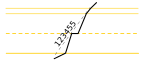
\includegraphics[width=\textwidth]{../img/kap5_approx_line}
	\caption{Strategie umisťující čísla vlaků na aproximovanou čáru}
	\label{fig:kap5:strategy_aproximation}
\end{figure}

Předpokládejme, že vedle této strategie budeme vytvářet segmenty představující horizontální pruhy kolem dopravních bodů, do kterých nějaká další strategie bude umisťovat kóty. Implementace naší strategie se bude snažit předejít situaci, kdy by se číslo vlaku překrývalo s~kótou z~těchto segmentů.

Pro přidávání zobrazitelných prvků do strategie nám bude stačit \linebreak \texttt{BasicStrategyManager} pracující s~\texttt{TPlacementType} a~\texttt{TSegmentType}. V~naší implementaci totiž nemusíme přidávat vlastní segmenty pro umístění čísel vlaku do třídy \texttt{SegmentRegistry}, která je součástí \texttt{StrategyManager}. Bude nám pouze stačit, když uvedeme v~\texttt{TPlacementType} dvě instance \texttt{Track}, mezi jejichž vizualizaci se umístí číslo vlaku. \texttt{TPlacementType} se pak převede pomocí bodů \texttt{TrainPath} na \texttt{TSegmentType}, který bude jako typ obsahovat dva segmenty pro umístění kót kolem instancí dodaných kolejí. V~ohraničení segmentů se vytvoří aproximovaná čára průběhu jízdy vlaku.

Nalezení aproximované čáry i~správného umístění čísla vlaku přenecháme implementaci \texttt{IStrategyDocker}, jejíž instanci vytvoříme pro každý vlak zvlášť. Konstruktoru dockeru předáme \texttt{TrainPath} obsahující body vytvářející průběh jízdy vlaku. Pomocí ní spolu se segmenty je docker schopný určit směr jízdy vlaku a~zároveň tak i~aproximovanou čáru s~umístěním čísla vlaku. Nyní bychom pro každé ze dvou možných umístění, nacházejících se na obrázku \ref{fig:kap5:strategy_aproximation_methods}, vytvořili metodu k umístění prvku. Přesnou implementaci metody pro situaci (a) si nyní detailně popíšeme.

\begin{figure}[!hbt]
	\centering
	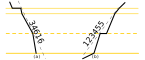
\includegraphics[width=.8\textwidth]{../img/kap5_approx_lines_two_types}
	\caption{Různé možnosti vytvoření aproximované čáry s~umístěním čísla vlaku}
	\label{fig:kap5:strategy_aproximation_methods}
\end{figure}

Strategii implementujeme tak, že se číslo vlaku umístí na prostředek aproximující čáry v~ohraničeném úseku segmenty pro kóty. Budeme chtít dosáhnout stavu na obrázku \ref{fig:kap5:strategy_aproximation_placement}, kdy horní levý vrchol prvku není umístěný na aproximující čáře, ale je přemístěný tak, aby se po rotaci nacházela jeho spodní hrana na aproximující čáře.

\begin{figure}[!hbt]
	\centering
	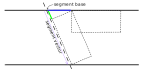
\includegraphics[width=.8\textwidth]{../img/kap5_strategy_implementation}
	\caption{Konečná pozice prvku určená strategií}
	\label{fig:kap5:strategy_aproximation_placement}
\end{figure}

\subsubsection*{Transformace velikosti prvku}
Budeme očekávat, že získáme dva body na aproximující čáře, které se budou zároveň nacházet na ohraničení segmenty pro kóty. Rozdílem těchto dvou bodů získáme vektor \texttt{segment vector} ve směru jízdy vlaku. Jeden z~těchto dvou bodů, který se nachází jako první ve směru jízdy vlaku, nazveme \texttt{segment base}. Nejdříve změříme \texttt{MeasureOverride()} velikost prvku \texttt{DesiredSize}, kterou mu přiřadíme v~\texttt{Arrange()}. V~případě, že délka prvku přesahuje délku \texttt{segment vector}, zapamatujeme si poměr rozdílu velikostí do proměnné \texttt{scale}. Dále by hrozilo, že prvek výškou bude i~po vynásobení \texttt{scale} zasahovat mimo ohraničenou oblast. Změříme proto délku odvěsny, vyznačenou zeleně na obrázku \ref{fig:kap5:strategy_aproximation_placement}, s~novou výškou prvku přenásobenou \texttt{scale}. Pro měření a~výpočty existují statické metody v~třídě \texttt{PlacementUtils}. Délka odvěsny by se vypočítala metodou \texttt{ComputeLegLength()}. Pokud součet délky odvěsny a~délky prvku bude přesahovat délku \texttt{segment vector}, jejich poměr vynásobíme s~původní hodnotou \texttt{scale}. Na prvku zavoláme \texttt{Scale()} s~nově vynásobenou hodnotou \texttt{scale}. Nyní pracujeme případně se zmenšeným prvkem, který se vejde do vyhrazeného místa.

\subsubsection*{Umístění a~transformace rotací}
Nyní provedeme samotné umístění -- aplikujeme přesun prvku s~rotací. \linebreak Nejdříve vypočítáme přesun prvku pomocí délky zelené odvěsny a~modré přepony z~obrázku \ref{fig:kap5:strategy_aproximation_placement}, pro škálovanou velikost prvku, která odpovídá vlastnostem prvku \texttt{ContentWidth} a~\texttt{ContentHeight}. Jako výchozí bod pro umístění použijeme \texttt{segment base}. Na horizontální ose k~němu přičteme součet délky modré přepony a~polovinu tloušťky čáry \texttt{LinePaint}, aby se s~ní číslo vlaku nepřekrývalo. Vertikální umístění bodu vypočítáme posunem od \texttt{segment base} po \texttt{segment vector} metodou \texttt{MoveInLine()} udáním délky posunu. Pokud je délka menší, do posunu započítáme polovinu volného prostoru, aby se prvek umístil na prostředek čáry. Takto jsme získali umístění, na které prvek přemístíme pomocí \texttt{Reposition()} metody. Protože se rotace aplikuje po směru hodinových ručiček, předáme \texttt{Rotate()} metodě ostrý úhel, který svírá \texttt{segment vector} a~horizontální čára.

\subsection*{Přesouvání obsahu mezi vrstvami a~jejich hit-testování}
Nyní si na příkladu výběru vlaku k~editaci ukážeme, jak implementovat přesun obsahu nákresného jízdního řádu do jiné vrstvy a~jak s~vrstvami pracovat. Předpokládejme, že máme view model \texttt{TrafficView}, který obsahuje seznam všech vlaků rozšířeného modelu se strategiemi, v~rámci kterého se umisťují vedle šikmé čáry průběhu jízdy vlaku kóty. Pokud například uživatel klikne na kótu, pomocí \textit{data bindingu} zmíněného v~\ref{kap4:observable_object} se zobrazí v~nějakém uživatelském prvku doplňující textové informace, které jsou kótou vizualizovány. Pokud se však rozhodne uživatel vybrat vlak k~editaci, přesune se jeho čára průběhu jízdy vlaku i~kóty spojené s~vlakem do popředí. Při editaci vlaku by pak bylo možné při kliknutí na kótu editovat informace spojené s~kótou z~jiného prvku uživatelského rozhraní.

Nejdříve implementujme přesunutí editovaného vlaku do vrstvy, která bude umístěna v~popředí. Vrstvu umístíme pomocí \texttt{AddOnCurrentTop()} do instance \texttt{DrawingManager}. Ve vrstvě bude metoda \texttt{ProvideVisuals()} poskytovat editovaný view model vlaku. Tomu umístíme na vrch zásobníku pomocí \linebreak \texttt{PushDrawingLayer()} tuto vrstvu. Rekurzivně se tato metoda ve view modelu vlaku zavolá na každý prvek z~\texttt{ProvideVisualsInSameLayer()}. Celý strom \linebreak těchto prvků je pak umístěn v~nové vrstvě. Pro navrácení těchto prvků do původní vrstvy použijeme na view modelu vlaku opačně \texttt{PopDrawingLayer()}.

Dále si popíšeme, jak implementovat klikání na zobrazitelné prvky. Předpokládejme, že budeme chtít z úspěšně otestovaných prvků v hit-testu získat pouze instance třídy \texttt{TimeComponent} představující kóty. Textové informace kóty vykreslené na vrchu chceme ve vedlejším prvku uživatelského rozhraní zobrazovat a~případně upravovat. Na instanci třídy \texttt{HitTestManager} se zavolá metoda \texttt{HitTest()} vůči vybranému bodu na prvek \texttt{TrafficView}, která projde podstrom prvků tohoto view modelu ve všech vrstvách. Získanou sekvenci úspěšně otestovaných prvků typu \texttt{TimeComponent} uložíme v~seznamu v~metodě delegáta \texttt{HitTestResultCallback}, který pak následně seřadíme podle vrstev \linebreak v~\texttt{OrderByLayers()} a~vybereme poslední prvek z~první vrstvy v pořadí. Ten se vykreslí jako poslední a jedná se o~kótu nacházející se na vrchu.